%% ****** Start of file apstemplate.tex ****** %
%%
%%
%%   This file is part of the APS files in the REVTeX 4 distribution.
%%   Version 4.1 of REVTeX, October 2009
%%
%%
%%   Copyright (c) 2001, 2009 The American Physical Society.
%%
%%   See the REVTeX 4 README file for restrictions and more information.
%%
%
% This is a template for producing manuscripts for use with REVTEX 4.0
% Copy this file to another name and then work on that file.
% That way, you always have this original template file to us.
%
% Group addresses by affiliation; use superscriptaddress for long
% author lists, or if there are many overlapping affiliations.
% For Phys. Rev. appearance, change preprint to twocolumn.
% Choose pra, prb, prc, prd, pre, prl, prstab, prstper, or rmp for journal
%  Add 'draft' option to mark overfull boxes with black boxes
%  Add 'showpacs' option to make PACS codes appear
%  Add 'showkeys' option to make keywords appear
\documentclass[useAMS,usenatbib]{mn2e}
%\documentclass[aps,prd,preprint,groupedaddress]{revtex4}
%\documentclass[aps,prl,preprint,superscriptaddress]{revtex4-1}
%\documentclass[aps,prl,reprint,groupedaddress]{revtex4-1}
\usepackage{natbib}
\usepackage{graphicx}
\usepackage[T1]{fontenc}
\usepackage{aecompl}
\usepackage{xr}
\usepackage{subfigure}
%\usepackage{graphicx,subfig}

% You should use BibTeX and apsrev.bst for references
% Choosing a journal automatically selects the correct APS
% BibTeX style file (bst file), so only uncomment the line
% below if necessary.
%\bibliographystyle{apsrev4-1}

% Psfig/TeX Release 1.2
% dvips version
%
% All software, documentation, and related files in this distribution of
% psfig/tex are Copyright 1987, 1988 Trevor J. Darrell
%
% Permission is granted for use and non-profit distribution of psfig/tex 
% providing that this notice be clearly maintained, but the right to
% distribute any portion of psfig/tex for profit or as part of any commercial
% product is specifically reserved for the author.
%
% $Header: psfig.tex,v 1.9 88/01/08 17:42:01 trevor Exp $
% $Source: $
%
% Thanks to Greg Hager (GDH) and Ned Batchelder for their contributions
% to this project.
%
\catcode`\@=11\relax
\newwrite\@unused
\def\typeout#1{{\let\protect\string\immediate\write\@unused{#1}}}
\typeout{psfig/tex 1.2-dvips}


%% Here's how you define your figure path.  Should be set up with null
%% default and a user useable definition.

\def\figurepath{./}
\def\psfigurepath#1{\edef\figurepath{#1}}

%
% @psdo control structure -- similar to Latex @for.
% I redefined these with different names so that psfig can
% be used with TeX as well as LaTeX, and so that it will not 
% be vunerable to future changes in LaTeX's internal
% control structure,
%
\def\@nnil{\@nil}
\def\@empty{}
\def\@psdonoop#1\@@#2#3{}
\def\@psdo#1:=#2\do#3{\edef\@psdotmp{#2}\ifx\@psdotmp\@empty \else
    \expandafter\@psdoloop#2,\@nil,\@nil\@@#1{#3}\fi}
\def\@psdoloop#1,#2,#3\@@#4#5{\def#4{#1}\ifx #4\@nnil \else
       #5\def#4{#2}\ifx #4\@nnil \else#5\@ipsdoloop #3\@@#4{#5}\fi\fi}
\def\@ipsdoloop#1,#2\@@#3#4{\def#3{#1}\ifx #3\@nnil 
       \let\@nextwhile=\@psdonoop \else
      #4\relax\let\@nextwhile=\@ipsdoloop\fi\@nextwhile#2\@@#3{#4}}
\def\@tpsdo#1:=#2\do#3{\xdef\@psdotmp{#2}\ifx\@psdotmp\@empty \else
    \@tpsdoloop#2\@nil\@nil\@@#1{#3}\fi}
\def\@tpsdoloop#1#2\@@#3#4{\def#3{#1}\ifx #3\@nnil 
       \let\@nextwhile=\@psdonoop \else
      #4\relax\let\@nextwhile=\@tpsdoloop\fi\@nextwhile#2\@@#3{#4}}
% 
%
\def\psdraft{
        \def\@psdraft{0}
        %\typeout{draft level now is \@psdraft \space . }
}
\def\psfull{
        \def\@psdraft{100}
        %\typeout{draft level now is \@psdraft \space . }
}
\psfull
\newif\if@prologfile
\newif\if@postlogfile
\newif\if@noisy
\def\pssilent{
        \@noisyfalse
}
\def\psnoisy{
        \@noisytrue
}
\psnoisy
%%% These are for the option list.
%%% A specification of the form a = b maps to calling \@p@@sa{b}
\newif\if@bbllx
\newif\if@bblly
\newif\if@bburx
\newif\if@bbury
\newif\if@height
\newif\if@width
\newif\if@rheight
\newif\if@rwidth
\newif\if@clip
\newif\if@verbose
\def\@p@@sclip#1{\@cliptrue}

%%% GDH 7/26/87 -- changed so that it first looks in the local directory,
%%% then in a specified global directory for the ps file.

\def\@p@@sfile#1{\def\@p@sfile{null}%
                \openin1=#1
                \ifeof1\closein1%
                       \openin1=\figurepath#1
                        \ifeof1\typeout{Error, File #1 not found}
                        \else\closein1
                            \edef\@p@sfile{\figurepath#1}%
                        \fi%
                 \else\closein1%
                       \def\@p@sfile{#1}%
                 \fi}
\def\@p@@sfigure#1{\def\@p@sfile{null}%
                \openin1=#1
                \ifeof1\closein1%
                       \openin1=\figurepath#1
                        \ifeof1\typeout{Error, File #1 not found}
                        \else\closein1
                            \def\@p@sfile{\figurepath#1}%
                        \fi%
                 \else\closein1%
                       \def\@p@sfile{#1}%
                 \fi}

\def\@p@@sbbllx#1{
                %\typeout{bbllx is #1}
                \@bbllxtrue
                \dimen100=#1
                \edef\@p@sbbllx{\number\dimen100}
}
\def\@p@@sbblly#1{
                %\typeout{bblly is #1}
                \@bbllytrue
                \dimen100=#1
                \edef\@p@sbblly{\number\dimen100}
}
\def\@p@@sbburx#1{
                %\typeout{bburx is #1}
                \@bburxtrue
                \dimen100=#1
                \edef\@p@sbburx{\number\dimen100}
}
\def\@p@@sbbury#1{
                %\typeout{bbury is #1}
                \@bburytrue
                \dimen100=#1
                \edef\@p@sbbury{\number\dimen100}
}
\def\@p@@sheight#1{
                \@heighttrue
                \dimen100=#1
                \edef\@p@sheight{\number\dimen100}
                %\typeout{Height is \@p@sheight}
}
\def\@p@@swidth#1{
                %\typeout{Width is #1}
                \@widthtrue
                \dimen100=#1
                \edef\@p@swidth{\number\dimen100}
}
\def\@p@@srheight#1{
                %\typeout{Reserved height is #1}
                \@rheighttrue
                \dimen100=#1
                \edef\@p@srheight{\number\dimen100}
}
\def\@p@@srwidth#1{
                %\typeout{Reserved width is #1}
                \@rwidthtrue
                \dimen100=#1
                \edef\@p@srwidth{\number\dimen100}
}
\def\@p@@ssilent#1{ 
                \@verbosefalse
}
\def\@p@@sprolog#1{\@prologfiletrue\def\@prologfileval{#1}}
\def\@p@@spostlog#1{\@postlogfiletrue\def\@postlogfileval{#1}}
\def\@cs@name#1{\csname #1\endcsname}
\def\@setparms#1=#2,{\@cs@name{@p@@s#1}{#2}}
%
% initialize the defaults (size the size of the figure)
%
\def\ps@init@parms{
                \@bbllxfalse \@bbllyfalse
                \@bburxfalse \@bburyfalse
                \@heightfalse \@widthfalse
                \@rheightfalse \@rwidthfalse
                \def\@p@sbbllx{}\def\@p@sbblly{}
                \def\@p@sbburx{}\def\@p@sbbury{}
                \def\@p@sheight{}\def\@p@swidth{}
                \def\@p@srheight{}\def\@p@srwidth{}
                \def\@p@sfile{}
                \def\@p@scost{10}
                \def\@sc{}
                \@prologfilefalse
                \@postlogfilefalse
                \@clipfalse
                \if@noisy
                        \@verbosetrue
                \else
                        \@verbosefalse
                \fi
}
%
% Go through the options setting things up.
%
\def\parse@ps@parms#1{
                \@psdo\@psfiga:=#1\do
                   {\expandafter\@setparms\@psfiga,}}
%
% Compute bb height and width
%
\newif\ifno@bb
\newif\ifnot@eof
\newread\ps@stream
\def\bb@missing{
        \if@verbose{
                \typeout{psfig: searching \@p@sfile \space  for bounding box}
        }\fi
        \openin\ps@stream=\@p@sfile
        \no@bbtrue
        \not@eoftrue
        \catcode`\%=12
        \loop
                \read\ps@stream to \line@in
                \global\toks200=\expandafter{\line@in}
                \ifeof\ps@stream \not@eoffalse \fi
                %\typeout{ looking at :: \the\toks200 }
                \@bbtest{\toks200}
                \if@bbmatch\not@eoffalse\expandafter\bb@cull\the\toks200\fi
        \ifnot@eof \repeat
        \catcode`\%=14
}       
\catcode`\%=12
\newif\if@bbmatch
\def\@bbtest#1{\expandafter\@a@\the#1%%BoundingBox:\@bbtest\@a@}
\long\def\@a@#1%%BoundingBox:#2#3\@a@{\ifx\@bbtest#2\@bbmatchfalse\else\@bbmatchtrue\fi}
\long\def\bb@cull#1 #2 #3 #4 #5 {
        \dimen100=#2 bp\edef\@p@sbbllx{\number\dimen100}
        \dimen100=#3 bp\edef\@p@sbblly{\number\dimen100}
        \dimen100=#4 bp\edef\@p@sbburx{\number\dimen100}
        \dimen100=#5 bp\edef\@p@sbbury{\number\dimen100}
        \no@bbfalse
}
\catcode`\%=14
%
\def\compute@bb{
                \no@bbfalse
                \if@bbllx \else \no@bbtrue \fi
                \if@bblly \else \no@bbtrue \fi
                \if@bburx \else \no@bbtrue \fi
                \if@bbury \else \no@bbtrue \fi
                \ifno@bb \bb@missing \fi
                \ifno@bb \typeout{FATAL ERROR: no bb supplied or found}
                        \no-bb-error
                \fi
                %
                \count203=\@p@sbburx
                \count204=\@p@sbbury
                \advance\count203 by -\@p@sbbllx
                \advance\count204 by -\@p@sbblly
                \edef\@bbw{\number\count203}
                \edef\@bbh{\number\count204}
                %\typeout{ bbh = \@bbh, bbw = \@bbw }
}
%
% \in@hundreds performs #1 * (#2 / #3) correct to the hundreds,
%       then leaves the result in @result
%
\def\in@hundreds#1#2#3{\count240=#2 \count241=#3
                     \count100=\count240        % 100 is first digit #2/#3
                     \divide\count100 by \count241
                     \count101=\count100
                     \multiply\count101 by \count241
                     \advance\count240 by -\count101
                     \multiply\count240 by 10
                     \count101=\count240        %101 is second digit of #2/#3
                     \divide\count101 by \count241
                     \count102=\count101
                     \multiply\count102 by \count241
                     \advance\count240 by -\count102
                     \multiply\count240 by 10
                     \count102=\count240        % 102 is the third digit
                     \divide\count102 by \count241
                     \count200=#1\count205=0
                     \count201=\count200
                        \multiply\count201 by \count100
                        \advance\count205 by \count201
                     \count201=\count200
                        \divide\count201 by 10
                        \multiply\count201 by \count101
                        \advance\count205 by \count201
                        %
                     \count201=\count200
                        \divide\count201 by 100
                        \multiply\count201 by \count102
                        \advance\count205 by \count201
                        %
                     \edef\@result{\number\count205}
}
\def\compute@wfromh{
                % computing : width = height * (bbw / bbh)
                \in@hundreds{\@p@sheight}{\@bbw}{\@bbh}
                %\typeout{ \@p@sheight * \@bbw / \@bbh, = \@result }
                \edef\@p@swidth{\@result}
                %\typeout{w from h: width is \@p@swidth}
}
\def\compute@hfromw{
                % computing : height = width * (bbh / bbw)
                \in@hundreds{\@p@swidth}{\@bbh}{\@bbw}
                %\typeout{ \@p@swidth * \@bbh / \@bbw = \@result }
                \edef\@p@sheight{\@result}
                %\typeout{h from w : height is \@p@sheight}
}
\def\compute@handw{
                \if@height 
                        \if@width
                        \else
                                \compute@wfromh
                        \fi
                \else 
                        \if@width
                                \compute@hfromw
                        \else
                                \edef\@p@sheight{\@bbh}
                                \edef\@p@swidth{\@bbw}
                        \fi
                \fi
}
\def\compute@resv{
                \if@rheight \else \edef\@p@srheight{\@p@sheight} \fi
                \if@rwidth \else \edef\@p@srwidth{\@p@swidth} \fi
}
%               
% Compute any missing values
\def\compute@sizes{
        \compute@bb
        \compute@handw
        \compute@resv
}
%
% \psfig
% usage : \psfig{file=, height=, width=, bbllx=, bblly=, bburx=, bbury=,
%                       rheight=, rwidth=, clip=}
%
% "clip=" is a switch and takes no value, but the `=' must be present.
\def\psfig#1{\vbox {
        % do a zero width hard space so that a single
        % \psfig in a centering enviornment will behave nicely
        %{\setbox0=\hbox{\ }\ \hskip-\wd0}
        %
        \ps@init@parms
        \parse@ps@parms{#1}
        \compute@sizes
        %
        \ifnum\@p@scost<\@psdraft{
                \if@verbose{
                        \typeout{psfig: including \@p@sfile \space }
                }\fi
                %
                \special{ps::[begin]    \@p@swidth \space \@p@sheight \space
                                \@p@sbbllx \space \@p@sbblly \space
                                \@p@sbburx \space \@p@sbbury \space
                                startTexFig \space }
                \if@clip{
                        \if@verbose{
                                \typeout{(clip)}
                        }\fi
                        \special{ps:: doclip \space }
                }\fi
                \if@prologfile
                    \special{ps: plotfile \@prologfileval \space } \fi
                \special{ps: plotfile \@p@sfile \space }
                \if@postlogfile
                    \special{ps: plotfile \@postlogfileval \space } \fi
                \special{ps::[end] endTexFig \space }
                % Create the vbox to reserve the space for the figure
                \vbox to \@p@srheight true sp{
                        \hbox to \@p@srwidth true sp{
                                \hss
                        }
                \vss
                }
        }\else{
                % draft figure, just reserve the space and print the
                % path name.
                \vbox to \@p@srheight true sp{
                \vss
                        \hbox to \@p@srwidth true sp{
                                \hss
                                \if@verbose{
                                        \@p@sfile
                                }\fi
                                \hss
                        }
                \vss
                }
        }\fi
}}
\def\psglobal{\typeout{psfig: PSGLOBAL is OBSOLETE; use psprint -m instead}}
\catcode`\@=12\relax


\def\ga{\mathrel{\mathchoice {\vcenter{\offinterlineskip\halign{\hfil
$\displaystyle##$\hfil\cr>\cr\sim\cr}}}
{\vcenter{\offinterlineskip\halign{\hfil$\textstyle##$\hfil\cr>\cr\sim\cr}}}
{\vcenter{\offinterlineskip\halign{\hfil$\scriptstyle##$\hfil\cr>\cr\sim\cr}}}
{\vcenter{\offinterlineskip\halign{\hfil$\scriptscriptstyle##$\hfil
\cr>\cr\sim\cr}}}}}
%
\def\la{\mathrel{\mathchoice {\vcenter{\offinterlineskip\halign{\hfil
$\displaystyle##$\hfil\cr<\cr\sim\cr}}}
{\vcenter{\offinterlineskip\halign{\hfil$\textstyle##$\hfil\cr<\cr\sim\cr}}}
{\vcenter{\offinterlineskip\halign{\hfil$\scriptstyle##$\hfil\cr<\cr\sim\cr}}}
{\vcenter{\offinterlineskip\halign{\hfil$\scriptscriptstyle##$\hfil
\cr<\cr\sim\cr}}}}}

\newcommand{\rtilde}{\tilde{r}}
\newcommand{\utilde}{\tilde{u}}


% \renewcommand{\topfraction}{.85}
% \renewcommand{\bottomfraction}{.7}
% \renewcommand{\textfraction}{.15}
% \renewcommand{\floatpagefraction}{.66}
% \renewcommand{\dbltopfraction}{.66}
% \renewcommand{\dblfloatpagefraction}{.66}

% Use the \preprint command to place your local institutional report
% number in the upper righthand corner of the title page in preprint mode.
% Multiple \preprint commands are allowed.
% Use the 'preprintnumbers' class option to override journal defaults
% to display numbers if necessary
%\preprint{}

%Title of paper
\title{Vlasolve: numerical method}

% repeat the \author .. \affiliation  etc. as needed
% \email, \thanks, \homepage, \altaffiliation all apply to the current
% author. Explanatory text should go in the []'s, actual e-mail
% address or url should go in the {}'s for \email and \homepage.
% Please use the appropriate macro foreach each type of information

% \affiliation command applies to all authors since the last
% \affiliation command. The \affiliation command should follow the
% other information
% \affiliation can be followed by \email, \homepage, \thanks as well.
\author[]{Sousbie, Thierry$^1$\\
\\
$^1$Institut d'Astrophysique de Paris, CNRS UMR 7095 and UPMC, 98bis, bd Arago, F-75014 Paris, France}
\begin{document}
\voffset -1cm
\date{\today}
\pagerange{\pageref{firstpage}--\pageref{lastpage}} \pubyear{2014}
\maketitle
\label{firstpage}
\begin{abstract}

\end{abstract}
\begin{keywords}
gravitation -- 
methods: numerical -- 
galaxies: kinematics and dynamics --
dark matter
\end{keywords}

%========================
%\section{Numerical implementation}
%========================
The evolution of the density distribution in a spherically symmetric dark matter halo is described by the Vlasov-poisson equation:
\begin{equation}
\frac{\partial f}{\partial t}+u\frac{\partial f}{\partial r}+\left(\frac{j^2}{r^3}-\frac{GM_r}{r^2}\right)\frac{\partial f}{\partial u},
\label{eq:vl}
\end{equation}
with $f=f\left(r,u,j,t\right)$ the phase-space distribution function at time $t$, distance to center $r$, radial velocity $u$ and angular momentum $j$, and $M_r=M\left(r^\prime<r\right)$ the mass inside a sphere of radius $r$.\\

In order to solve this equation numerically, we use a semi-Lagrangian method similar to \cite{Fuji83}. That is, phase space $\left(r,u,j\right)$ is discretized into a rectangular mesh that spans the domain of interest and the value of the initial distribution function is sampled at each mesh site $i$ with coordinates $\left(r_i,u_i,j_i\right)$. Considering each mesh site as a particle, the value of $f\left(r_i,u_i,j_i,t+dt\right)$ at site $i$ and time $t+dt$ can then be easily deduced by integrating the particle trajectory backward in time at time $t$ and interpolating the distribution function at that location.\\

 For each time step, the integration of the particle trajectory can be carried out using the fact that equation (\ref{eq:vl}) can be split \`{a} la \cite{CK} into a free-streaming part:
\begin{equation}
\frac{\partial f}{\partial t}+u\frac{\partial f}{\partial r}+\frac{j^2}{r^3}\frac{\partial f}{\partial u},
\label{eq:vl_fs}
\end{equation}
and an acceleration part:
\begin{equation}
\frac{\partial f}{\partial t}-\frac{GM_r}{r^2}\frac{\partial f}{\partial u}.
\label{eq:vl_acc}
\end{equation}
Indeed, combining equations (\ref{eq:vl_fs}) and (\ref{eq:vl_acc}) with a leap-frog type numerical integrator, the value of $f\left(r_i,u_i,j_i,t+dt\right)$ for each grid site can be deduced at a second order accuracy level from its value one time-step earlier, at time $t$, through a sequence of simple shifts:
\begin{eqnarray}
f^*\left(r_i,u_i,j_i\right) &=& f\left(\rtilde_i,\utilde_i,j_i,t,\right), \label{eq:leapfrog1}\\
f^{**}\left(r_i,u_i,j_i\right) &=& f^*\left(r,u-{GM_r}/{r^2}dt,j\right), \label{eq:leapfrog2}\\
f\left(r_i,u_i,j_i,t+dt\right) &=& f^{**}\left(\rtilde_i,\utilde_i,j_i\right), \label{eq:leapfrog3}
\end{eqnarray}

where $\left(\rtilde_i,\utilde_i\right)=\left(r_i\left(t-dt/2\right),u_i\left(t-dt/2\right)\right)$ is the position of grid site $i$ free streamed half a time step backward in time using equation (\ref{eq:vl_fs}), and $M_r$ is computed from $f^*\left(r_i,u_i,j_i\right)$. This integration scheme requires two interpolations per time step: a 2D\footnote{note that due to the spherical coordinates system, $\utilde_i \neq u_i$.} one in the $\left(r,u\right)$ sub-space for the free streaming part\footnote{equations (\ref{eq:leapfrog3}) and (\ref{eq:leapfrog1}) of the following time-step can indeed be combined into a single interpolation.} (\ref{eq:leapfrog1}) and a 1D interpolation for the acceleration part (\ref{eq:leapfrog2}). Similarly to \cite{Fuji83}, these interpolations are carried out using third order spline interpolation.\\

With such a technique, it is very important to carefully define the domain of integration so that it spans the smallest possible phase-space volume (i.e. it needs only contain any region where the distribution function will be non-null at any point in time), while maintaining an adequate resolution everywhere (i.e. phase space distribution features should keep an approximately constant resolution in terms of pixel independently of their position or orientation in phase space). Following \cite{Fuji83}, the computational domain is therefore defined as $\left(r,u,j\right)$ such that $R_{\rm min}\leq r\_{\rm max}$, $\left|u\right|\leq u_{\rm max}$ and $0\leq j \leq J_{\rm max}$ and the grid site have a linear distribution along $u$, a logarithmic distribution along $j$ and the positions of the $k^{\rm th}$ angular momentum site is $j_k=k^2\left(J_{\rm max}/{N_k}^2\right)$.\\

Using a logarithmic scale along the radial direction proves particularly advantageous as it allows resolving tiny features close to the center that will expand to larger scales later on as they get further away. One downside of it however is that a small sphere of radius $R_{\rm min}$ will necessarily be missing from the domain. This shortcoming is usually dealt with by considering the central part as a small reflecting spheres (see e.g. \cite {Gott73}, \cite{Fuji83}). Although simple, this method presents the major drawback of introducing a systematic shift in phase space distribution: particles reaching the reflective kernel boundary instantly travel the length $L$ through the part of their trajectory contained in the central region below $R_{\rm min}$. As a consequence, a particle $i$ reaching the kernel with velocity $u_i$ will systematically be spuriously shifted in time by $\delta t_u \approx u_i/L_i$ while another particle $j$ with velocity $v_j \neq u_i$ will systematically be shifted in time by $\delta t_v \approx v_j/L_j \neq \delta t_u$, introducing a systematic lag between orbits.\\

We remedy this issue by taking into account the time spent inside the central sphere for each particle reaching it. We first note that the only quantity that depends on time in equations (\ref{eq:leapfrog1}) through (\ref{eq:leapfrog3}) is $M_r=M\left(r^\prime \leq r\right)$, the mass below $r$, a strictly increasing function of the radius that tends to $0$ as $r$ decreases. For $r\leq R_{\rm min}$ sufficiently small, the influence of the acceleration part (\ref{eq:vl_acc}) of the split Vlasov equation over a particle with coordinates $\left(r_{\leq R_min},u\right)$ therefore becomes negligible compared to that of its free-streaming counterpart (\ref{eq:vl_fs}) and we can safely neglect the time dependence. As a consequence, under the assumption that $R_{\rm min}$ is sufficiently small, the trajectory followed by each grid site particle that penetrates into the central sphere does not depend on time, allowing us to pre-compute them for each grid site whose value at previous time step should be interpolated inside the central sphere.\\

From a technical point of view, this delayed central sphere method is implemented by associating a linked list to each grid site whose coordinates $\left(\rtilde_i,\utilde_i\right)$ half a time step backward in time is such that $\rtilde_i\leq R_{\rm min}$. Each linked list contains as many elements as the number of time steps necessary for the corresponding particle to travel throughout the central region and the $n^{th}$ element in the list stores the coordinates of its grid site $n$ time steps backward in time. Before starting the simulation, we initialize each element coordinate and corresponding value of the initial distribution function. For each time step, the value of each element is then simply updated by assigning to it the value of its successor while the last element value, whose coordinates fall outside the central region, is interpolated. A comparison of the results obtained with the reflective central sphere and our improved delayed central sphere is shown on figure \ref{fig:delayed}.\\

\begin{figure*}
\begin{minipage}[c]{\linewidth}
\begin{centering}
\subfigure[Reflective central sphere]{\centering 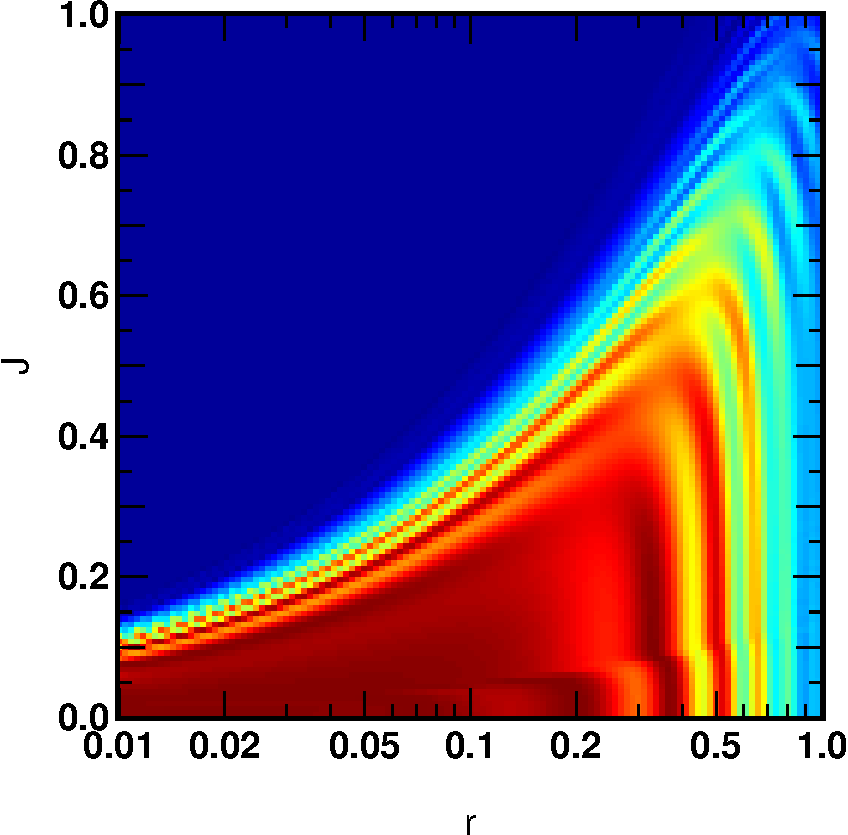
\includegraphics[width=0.49\linewidth]{fig/reflective.pdf}}
\subfigure[Delayed central sphere]{\centering 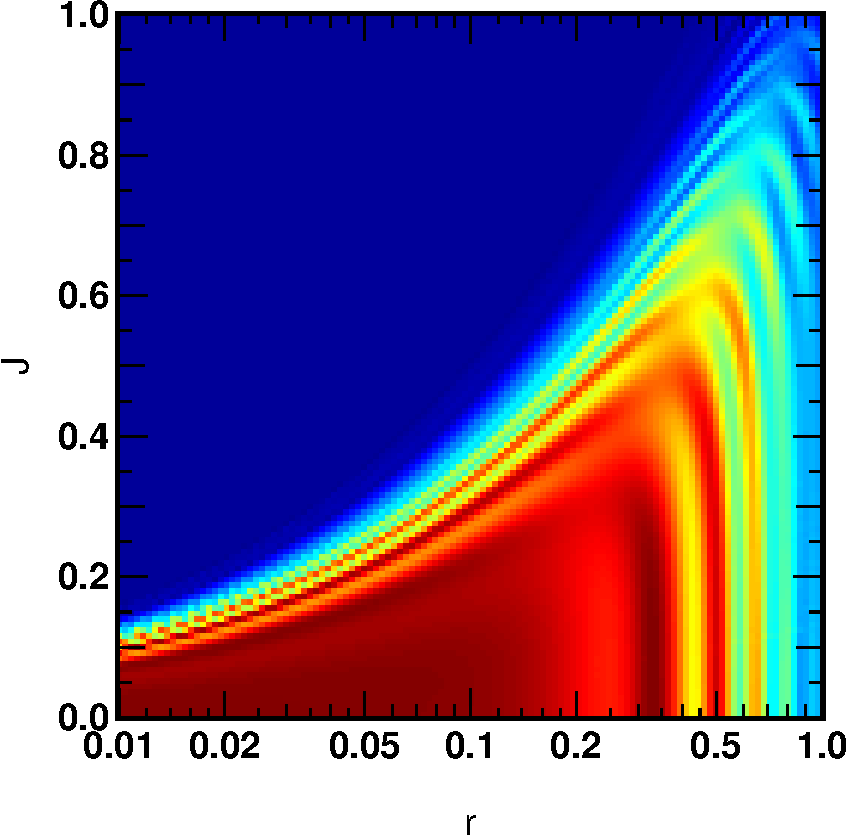
\includegraphics[width=0.49\linewidth]{fig/delayed.pdf}}
\caption{Comparison of the simulated evolution of a spherical top hat profile at $t=30$ in the $\left(r,u=0,j\right)$ plane, for a reflective central sphere (left) and our improved delayed central sphere (right). The systematic artificial speed increase undergone by orbits that penetrate the central region compared to their higher angular momentum counterparts can clearly be observed at low $j$ on the left picture where a reflective sphere is used, while the distribution function does not exhibit such spurious feature when a delayed kernel is used (right).}
\end{centering}
\end{minipage}
\label{fig:delayed}
\end{figure*}

We conclude this section with a word on parallelization. For the purpose of this work, we implemented a hybrid shared and distributed memory version of the algorithm described above via the OpenMP and MPI libraries respectively. Shared memory parallelism is relatively straightforward to implement in the spherically symmetric case, taking advantage of the fact that the angular momentum $j$ is a conserved quantity. Indeed, angular momentum conservation implies that that the spline interpolations required for the numerical integration steps (\ref{eq:leapfrog1}) through (\ref{eq:leapfrog3}) can be computed independently for each grid slice of constant $j$. We therefore easily reach an almost perfect\footnote{spline interpolation is by far the most time consuming computation in a time-step} parallelization up to a number of tasks equal to the grid resolution $N_j$ the dimension $j$, which is typically larger than the number of available cores present on a shared memory systems. 

Distributed memory parallelization via MPI is not as trivial though as in that case the total number of available computational cores may become very large while spline interpolations are intrinsically non-local, making it non trivial to split computations along dimensions other than $j$. Sticking with the trivial parallelization described above, the maximum total number of processes running in parallel is therefore limited to $N_j$, which may become an issue for simulations with high resolution in position and velocity but comparatively low resolution in angular momentum. We overcome this limitation by following \cite{Crouseilles09} who propose to localize cubic splines interpolation over large enough patches that may not cover the full integration domain along one or more dimensions.

%----------------------------------------------------------------------------
\begin{thebibliography}{}
%----------------------------------------------------------------------------
\bibitem[\protect\citeauthoryear{Cheng \& Knorr}{1976}]{CK} 
  Cheng C.~Z., Knorr G., 1976, JCoPh, 22, 330 
\bibitem[\protect\citeauthoryear{Crouseilles \& al.}{2009}]{Crouseilles09} 
  Crouseilles N., Latu G., Sonnendr\"{u}cker, E., 2009, JCoPh, 228, 1429  
\bibitem[\protect\citeauthoryear{Fujiwara}{1983}]{Fuji83} 
  Fujiwara T., 1983, PASJ, 35, 547 
\bibitem[\protect\citeauthoryear{Gott}{1973}]{Gott73} 
  Gott, J.R. III , 1973, ApJ, 186, 481 
\end{thebibliography}
\label{lastpage}
\end{document}


@ARTICLE{1983PASJ...35..547F,
   author = {{Fujiwara}, T.},
    title = "{Integration of the collisionless Boltzmann equation for spherical stellar systems}",
  journal = {\pasj},
 keywords = {Boltzmann-Vlasov Equation, Gravitational Collapse, Star Clusters, Star Distribution, Stellar Evolution, Stellar Motions, Stellar Systems, Celestial Mechanics, Distribution Functions, Jeans Theory, Numerical Integration, Relaxation (Mechanics), Spherical Plasmas},
     year = 1983,
   volume = 35,
    pages = {547-558},
   adsurl = {http://adsabs.harvard.edu/abs/1983PASJ...35..547F},
  adsnote = {Provided by the SAO/NASA Astrophysics Data System}
}

@ARTICLE{1976JCoPh..22..330C,
   author = {{Cheng}, C.~Z. and {Knorr}, G.},
    title = "{The integration of the Vlasov equation in configuration space}",
  journal = {Journal of Computational Physics},
 keywords = {Computer Programs, Digital Simulation, Magnetohydrodynamic Stability, Numerical Integration, Plasma Physics, Vlasov Equations, Collisionless Plasmas, Entropy, Fortran, Free Flow, Interpolation, Landau Damping, One Dimensional Flow, Run Time (Computers), Spline Functions},
     year = 1976,
    month = nov,
   volume = 22,
    pages = {330-351},
      doi = {10.1016/0021-9991(76)90053-X},
   adsurl = {http://adsabs.harvard.edu/abs/1976JCoPh..22..330C},
  adsnote = {Provided by the SAO/NASA Astrophysics Data System}
}

@article{Crouseilles:2009:PVS:1497640.1497961,
 author = {Crouseilles, Nicolas and Latu, Guillaume and Sonnendr\"{u}cker, Eric},
 title = {A Parallel Vlasov Solver Based on Local Cubic Spline Interpolation on Patches},
 journal = {J. Comput. Phys.},
 issue_date = {March, 2009},
 volume = {228},
 number = {5},
 month = mar,
 year = {2009},
 issn = {0021-9991},
 pages = {1429--1446},
 numpages = {18},
 url = {http://dx.doi.org/10.1016/j.jcp.2008.10.041},
 doi = {10.1016/j.jcp.2008.10.041},
 acmid = {1497961},
 publisher = {Academic Press Professional, Inc.},
 address = {San Diego, CA, USA},
 keywords = {Numerical methods, Parallelism, Semi-Lagrangian method, Vlasov equation},
} 

